% Configuración del tipo páginas
	\documentclass[11pt, a4paper,english,spanish]{article}
	\parindent = 11pt
	\parskip = 0 pt	
	\usepackage[width=15.5cm, left=3cm, top=2.5cm, height= 24.5cm]{geometry}

% Paquete para reconocer la separación en sílabas en español
	\usepackage[utf8]{inputenc}
	\usepackage[spanish]{babel}

% Paquetes especiales
	\usepackage{amsmath}
	\usepackage{amsthm} %paquete para teoremas y propiedades
	\usepackage{amsfonts}
	\usepackage{amssymb}
	\usepackage{upgreek}
	\usepackage{ifthen}
	\usepackage{alltt}
	\usepackage[pdftex]{graphicx}
  	\usepackage{textcomp}
	\usepackage{float}
	%\usepackage{dsfont}
	\usepackage{graphicx} %paquete para incluir imagenes

	\usepackage{caption}
	\usepackage{subcaption}

\usepackage{tabularx}
\usepackage{multirow}

\usepackage{algorithm}
\usepackage{algpseudocode}

% Paquete para incluir hypervinculos
	\usepackage{color}
	\usepackage{url}
	\definecolor{lnk}{rgb}{0,0,0.4}
	%colores para la inclusion del codigo
	\definecolor{gray97}{gray}{.97}
	\definecolor{gray75}{gray}{.75}
	\definecolor{gray45}{gray}{.45}
	\usepackage[colorlinks=true,linkcolor=lnk,citecolor=black,urlcolor=black]{hyperref}

	\newcommand{\todo}{\textbf{\textcolor{red}{TODO: }}}

% Paquete para armar índices
	\usepackage{makeidx}
	\makeindex

\renewcommand{\thefootnote}{\arabic{footnote}} %config de footnote

%Paquete y su config para incluir los codigos de python
\usepackage{times}
\usepackage{listings}
\lstset{ frame=Ltb,
framerule=0pt,
aboveskip=0.5cm,
framextopmargin=3pt,
framexbottommargin=3pt,
framexleftmargin=0.4cm,
framesep=0pt,
rulesep=.4pt,
backgroundcolor=\color{gray97},
rulesepcolor=\color{black},
%
stringstyle=\ttfamily,
showstringspaces = false,
basicstyle=\footnotesize\ttfamily,
commentstyle=\color{gray45},
keywordstyle=\bfseries,
language=python,
%
numbers=left,
numbersep=15pt,
numberstyle=\tiny,
numberfirstline = false,
breaklines=true,
}

\lstset{emph={%  
    size_t, clock_t%
    }, emphstyle={\bfseries}%
}%

% minimizar fragmentado de listados
\lstnewenvironment{listing}[1][]
{\lstset{#1}\pagebreak[0]}{\pagebreak[0]}

\lstdefinestyle{consola}
{basicstyle=\scriptsize\bf\ttfamily,
backgroundcolor=\color{gray75},
}

\lstdefinestyle{Python}
{language=Python}

\lstdefinestyle{bash}
{language=bash,
numbers=none}

	
% Carátula
	\usepackage{caratula}

\newcommand{\comment}[1]{\emph{// {#1}\;}} 
\newcommand{\la}{\(\leftarrow\)}
\newcommand{\ra}{\(\rightarrow\)}

\hypersetup{ 
pdfauthor = {},
pdftitle = {}, 
pdfkeywords = {},
pdfstartview={XYZ null null 0.80},
}

\begin{document}
\titulo{TP2}
%\subtitulo{Grupo ???}
%\resumen{
%	\textbf{Resumen: } \\ \\
%	\indent \textbf{Keywords: }
%}
\fecha{Fecha de entrega: 27/10/2016}
\materia{Redes Neuronales Artificiales}
\integrante{Panarello, Bernabé}{194/01}{bpanarello@gmail.com}
\integrante{Uhrich, Verónica}{021/10}{veronicauhrich@gmail.com}
\integrante{Villanueva, Paula}{701/10}{villanuevapaulasofia@gmail.com}

\maketitle
% Índice
\newpage 

\printindex 

\tableofcontents

\normalsize

\newpage
\section{Reducción de dimensiones}

\subsection{Introducción}

Disponemos de un dataset de Bag of Words (BOW) que representan descripciones de texto correspondientes a compañías Brasileras clasificadas en nueve categorías distintas. Cada BOW contiene 856 atributos correspondientes a frecuencias de palabras y, debido a la alta dimensionalidad, se busca reducir el conjunto de datos a 3 dimensiones mediante las reglas de aprendizaje de Oja y Sanger.

Regla Oja:
\begin{itemize}
	\item$\Delta W_{ij} = \eta (x_i - \widetilde{x_i}) y_j$
	\item$\widetilde{x_i} = \sum_{j=1}^m y_j . W_{ij}$, donde $m$ es la cantidad de outputs.
\end{itemize}

Regla Sanger:
\begin{itemize}
	\item$\Delta W_{ij} = \eta (x_i - \widetilde{x_i}) y_j$
	\item$\widetilde{x_i} = \sum_{k=1}^j y_k . W_{ik}$
\end{itemize}

\subsection{Modelo}

Cada entrada del dataset contiene 856 atributos, por lo tanto tenemos 856 unidades de entrada. Como queremos reducir el conjuntos de datos a 3 dimensiones, tenemos 3 unidades de salida.

\begin{itemize}
	\item$X \in \mathbb{R}^{856}$
	\item$Y \in \mathbb{R}^3$
	\item$W, \Delta W \in \mathbb{R}^{856\times 3}$
\end{itemize}

\begin{figure}[ht!]
	\centering
	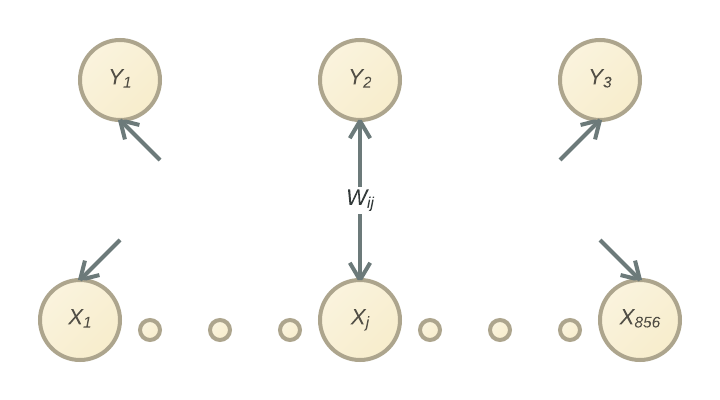
\includegraphics[width=0.7\linewidth]{img/parte1-modelo.png}

	\caption{Modelo de red}
\end{figure}

\subsection{Implementación}

\subsubsection{Prepocesamiento de datos}

El dataset se preprocesa centrando los datos en el 0, calculando la media de las frecuencias de cada palabra (posición del vector) y restándosela a cada una de ellas. De esta forma, la media de cada columna del dataset resultante es 0 y los datos quedan distribuidos alrededor del 0.

\subsubsection{Pseudocódigo}

Inicializamos la matriz de pesos con valores random $\in[-1/2, 1/2]$.

\begin{algorithm}[H]
\caption{train}
\begin{algorithmic}
	\State e = 0
    \While {not fin}
        \State e+=1
        \State lr = lrcons * e$^{-1}$
        \For {x in dataset}
            \State y = x $\bullet$ weights
            \State aplicamos regla
            \State weights += dw
        \EndFor
    \EndWhile
    \State return weights
\end{algorithmic}
\end{algorithm}

\begin{algorithm}[H]
\caption{fin}
\begin{algorithmic}
	\State return (e == max\_epochs) or (weights es ortogonal)
\end{algorithmic}
\end{algorithm}

\begin{algorithm}[H]
\caption{ortogonal}
\begin{algorithmic}
	\State return (weigths$^t$ $\bullet$ weights) - identity matrix $<$ epsilon * identity matrix
\end{algorithmic}
\end{algorithm}


\subsection{Ejecución}

\subsubsection{Modo de uso}

\subsubsection{Requerimientos}

Python

Numpy, Matplotlib

\newpage
\newpage
\section{Eficiencia energética}

%%--------------------------------------------------------------------------------------------------------------------------------------------------

\subsection{Introducción}

%%--------------------------------------------------------------------------------------------------------------------------------------------------

\subsection{Modelo}

Se probaron varias arquitecturas de red, incluyendo una con nivel más de profundidad respecto a la del punto 1, pero finalmente nos quedamos con la de 3 niveles (una capa oculta).

{
"layers": [{
"type": "input",
"size": 8
}, {
"type": "sigmoid",
"size": 20,
"beta": 20
}, {
"type": "tanh",
"size": 2,
"beta": 20
}]
}


\begin{figure}[ht!]
	\centering
	\includegraphics[width=1\linewidth]{fig/parte2-modelo.jpg}
	\caption{Modelo de la red}
\end{figure}

Se colocaron a la salida dos unidades del tipo tanh, cada una representando uno de los valores de salida a aproximar (energía y lo otro). Se utilizó tanh (x) 
dado que aproxima bastante a una recta dentro del codiminio (-1,1). Se utilizó la activación tanh(z / beta).  El valor beta nos permite ajustar la pendiente de la curva. 
Pendientes mas bajas aceleran el entrenamiento.



%%--------------------------------------------------------------------------------------------------------------------------------------------------

\subsection{Implementación}

Overfitting: El otro problema que encaramos es que, cuando el error de entrenamiento absoluto llega a bajar a cierto valor (aproximadamente 0.06, dependiendo de los parámetros), 
el error de testeo comienza a incrementarse (llega a un mínimo de 0.1 aproximadamente) y nunca baja. Intentamos palear esto incrementando el parámetro de regularización, pero no resultó.

\subsubsection{Prepocesamiento de datos}

Los datos pertenecientes al dataset fueron normalizados mediante la siguiente fórmula: 

\begin{align*}
		\frac{x - \mu}{max(features) - min(features)} 
\end{align*}

donde $x$ perteneces a features, y $\mu$ es la media de los features. Esto se hizo para que todos los datos  del dataset queden en el rango (-1,1).

\subsubsection{Pseudocódigo}

%%--------------------------------------------------------------------------------------------------------------------------------------------------

\subsection{Ejecución}

\subsubsection{Modo de uso}

\textbf{Para entrenar las redes:}

\noindent\texttt{\scriptsize{python trainnet1.py -m ej1.lmodel -o redentrenada1.params -t 3000 -e 0.01 -l 0.005 -b 1}} \\

\texttt{\scriptsize{-x tp1\_ej1\_training.csv}} \\

\noindent\texttt{\scriptsize{python predict2.py -m ej2.lmodel -p redentrenada2.params -x tp1\_ej2\_testing.csv}} \\





\subsubsection{Requerimientos}

%%--------------------------------------------------------------------------------------------------------------------------------------------------

\subsection{Resultados}

Probando combinaciones de $\beta$, learning rate y el término de regularización, lo mejor que pudimos lograr fue:

\begin{itemize}
	\item Error absoluto promedio de testing: 0.033. Esto es, promediando las distancias euclidianas entre el vector de dos posiciones predicho y el verdadero. 
	\item Error relativo promedio: 0.38 (38$\%$). Esto es la desviación relativa promedio de los valores verdaderos, tomado como el error absoluto / error promedio.
\end{itemize}

Como podemos ver, la estimación hasta el momento es bastante mala.

%%--------------------------------------------------------------------------------------------------------------------------------------------------

\subsection{Conclusiones}


\section{Código fuente}

\subsection{Carga de datos}

\lstinputlisting[language=Python]{../data_loader.py}

\subsection{Ejercicio 1}

\subsubsection{Entrenamiento}

\lstinputlisting[language=Python]{../hbtrain.py}

\subsubsection{Ploteo}

\lstinputlisting[language=Python]{../hbplot.py}

\subsubsection{Reducción}

\lstinputlisting[language=Python]{../hbreduction.py}

\subsubsection{Learning}

\lstinputlisting[language=Python]{../us_learning.py}

\subsubsection{Testeo}

\lstinputlisting[language=Python]{../tests1.py}

\subsection{Ejercicio 2}

\subsubsection{Entrenamiento}

\lstinputlisting[language=Python]{../khtrain.py}

\subsubsection{Visualizador de mapa generado}

\lstinputlisting[language=Python]{../khdispplaymap.py}

\subsubsection{Clasificador de ejemplos}

\lstinputlisting[language=Python]{../khclassify.py}

\subsubsection{Heap map}

\lstinputlisting[language=Python]{../heat_map.py}

\subsubsection{Kohonen}

\lstinputlisting[language=Python]{../kohonen.py}

Mapeo de categorías:

\lstinputlisting[language=Python]{../kohonen_category_mapper.py}

Clasificador:

\lstinputlisting[language=Python]{../kohonen_classifier.py}

\subsubsection{Parámetros}

\lstinputlisting[language=Python]{../params_io.py}

\appendix

\end{document}
